\section{NetHack Learning Environment}
\label{nethack}

The NetHack Learning Environment (NLE)~\citep{kuttler2020nethack} is a scalable, procedurally generated, stochastic, rich, and challenging environment designed to drive long-term research in RL on problems such as exploration, planning, skill acquisition, and language-conditioned RL. Built around the classic and highly complex terminal roguelike game NetHack, NLE provides a complex and dynamic environment where agents must navigate through procedurally generated dungeons, interact with hundreds of entity types, and learn to overcome various challenges. 

The goal of the player is to descend through procedurally generated dungeon levels while killing monsters, solving puzzles, and gathering better equipment in order to retrieve the Amulet of Yendor and finally ascend back to the surface to win the game. 
NetHack is notoriously challenging, even for human players. Mastering the game can take years even with online resources like the NetHack Wiki. Success in NetHack demands long-term strategic planning, as a winning game can involve hundreds of thousands of steps, as well as short-term tactics to fight hordes of monsters. Accurate credit assignment is also crucial to understanding which actions contributed to success or failure. NetHack has already been used extensively as a testbed for RL agents~\citep{wolczyk2024fine, piterbarg2023diff, hambro2022dungeons}; tabula-rasa RL agents particularly struggle due to sparse reward, complex credit assignment, extremely long-time-horizon, and high stochasticity of the game. The current state-of-the-art agent still remains a hand-coded symbolic policy \citep{hambro2022insights}.

\label{nethack_language_wrapper}
\subsection{NetHack Language Wrapper}
The NetHack Language Wrapper \citep{goodger2023nethack} is a tool designed to interface with the NLE and MiniHack by translating non-language observations into text-based representations. This wrapper, converts various NLE observations such as \verb|glyphs|, \verb|blstats|, \verb|tty_chars|, \verb|inv_letters|, \verb|inv_strs|, and \verb|tty_cursor| into readable text equivalents. For example, it transforms the visual display of the game environment into a textual description, including details about the surroundings, inventory, and player statistics. The wrapper also supports text-based actions, allowing users to interact with the environment using commands like \verb|wait|, \verb|apply|, and \verb|north|, which are then converted into the discrete actions required by the NLE. This functionality enables easier interaction with the NetHack environment, particularly for language models.

\begin{figure}[h]
    \centering
    \begin{subfigure}[b]{0.48\textwidth}
        \centering
        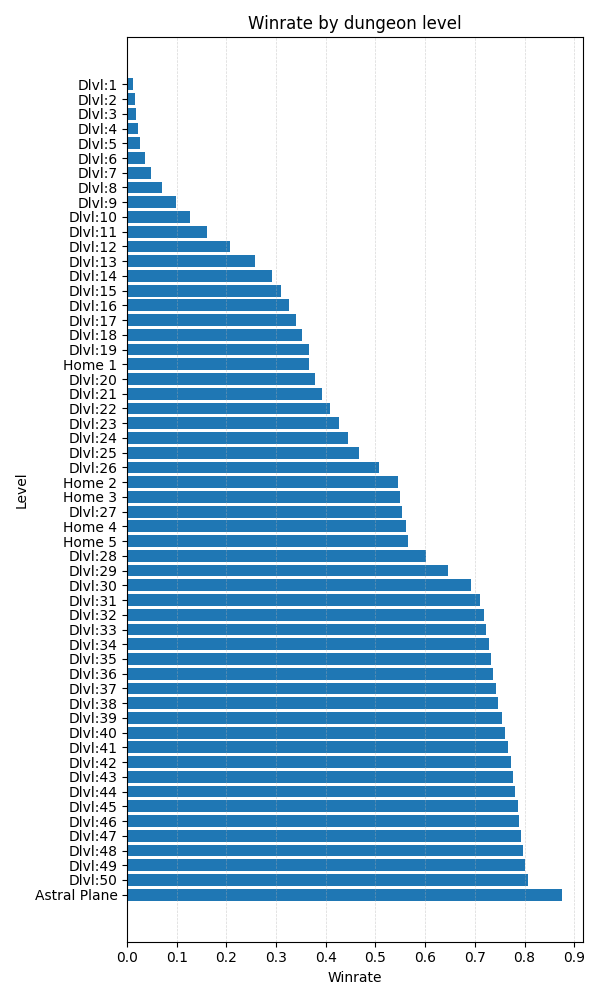
\includegraphics[width=\textwidth]{iclr2025/images/dungeon_levels.png}
        \caption{NetHack progression by dungeon level reached}
    \end{subfigure}
    \hfill
    \begin{subfigure}[b]{0.48\textwidth}
        \centering
        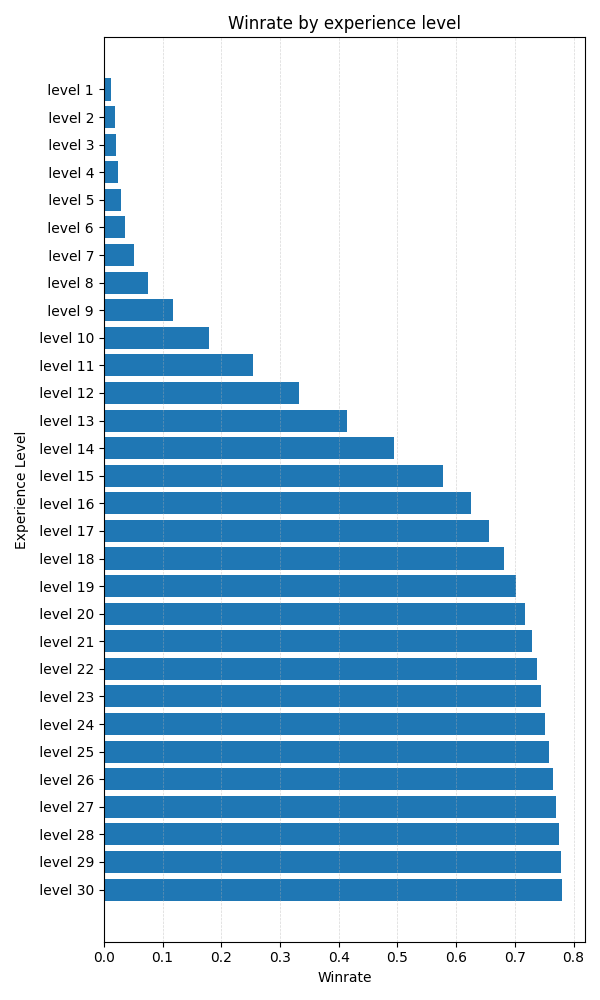
\includegraphics[width=\textwidth]{iclr2025/images/experience_levels.png}
        \caption{NetHack progression by experience level}
    \end{subfigure}
    \caption{}
    \label{NLE_progression}
\end{figure}

\subsection{New NetHack Progression System}
NetHack features an in-game scoring system that rewards players for actions such as killing monsters, identifying objects, eating food, collecting gold and items, and ultimately ascending in the game. However, we argue that this scoring system does not effectively capture true game progression, as players can win the game with scores ranging from a few hundred thousand to several million points. To address this limitation, we developed a novel, data-informed progression metric using a dataset of human-played NetHack games \citep{hambro2022dungeons}. Specifically, we recorded the dungeon levels and experience levels achieved in each game, as well as whether the game resulted in an ascension. Utilizing these statistics, we constructed a data-centric progression system where each data point represents the probability of a human player winning the game after reaching a specific dungeon level or experience level. The resulting progression curves are presented in Figure \ref{NLE_progression}. For practical purposes, we define Dungeon Level 1 (Dlvl:1) and Experience Level 1 as representing 0\% progression, corresponding to the game's starting point, and ascension as 100\% progression. The agent's overall progress is thus determined by the highest progression achieved between the dungeon level and experience level attained.

\label{NetHack-progression-metric}



\subsection{NetHack Results}
We provide NetHack results for LLM and VLM mode in Tables~\ref{LLM_NLE} and~\ref{VLM_NLE}. Standard errors are computed using 5 seeds. o1-preview achieves the highest progression out of all the tested models. However, it is still very far from making any significant progression in the game. The best individual run was achieved by Gemini-1.5-Pro vision-language mode, reaching dungeon level 3 and experience level 4.

\begin{table}[h]
    \centering
    \begin{minipage}[t]{0.48\linewidth}
    \centering
    \caption{LLM Performance on nle}
    \begin{tabular}{lc}
    \hline
    Model & Average Progress (\%) \\
    \hline
    o1-preview & 1.57 $\pm$ 0.40 \\
    claude-3.5-haiku & 1.16 $\pm$ 0.42 \\
    claude-3.5-sonnet & 0.58 $\pm$ 0.52 \\
    gpt-4o & 0.37 $\pm$ 0.37 \\
    gemini-1.5-pro & 0.37 $\pm$ 0.37 \\
    llama-3.1-70b-it & 0.35 $\pm$ 0.35 \\
    gpt-4o-mini & 0.00 $\pm$ 0.00 \\
    gemini-1.5-flash & 0.00 $\pm$ 0.00 \\
    llama-3.2-1b-it & 0.00 $\pm$ 0.00 \\
    llama-3.2-3b-it & 0.00 $\pm$ 0.00 \\
    llama-3.1-8b-it & 0.00 $\pm$ 0.00 \\
    llama-3.2-11b-it & 0.00 $\pm$ 0.00 \\
    llama-3.2-90b-it & 0.00 $\pm$ 0.00 \\
    \hline
    \label{LLM_NLE}
    \end{tabular}
    \end{minipage}
    \hfill
    \begin{minipage}[t]{0.48\linewidth}
    \centering
    \caption{VLM Performance on nle}
    \begin{tabular}{lc}
    \hline
    Model & Average Progress (\%) \\
    \hline
    claude-3.5-sonnet & 1.16 $\pm$ 0.42 \\
    gemini-1.5-pro & 0.48 $\pm$ 0.48 \\
    gpt-4o & 0.37 $\pm$ 0.37 \\
    gpt-4o-mini & 0.00 $\pm$ 0.00 \\
    gemini-1.5-flash & 0.00 $\pm$ 0.00 \\
    llama-3.2-11b-it & 0.00 $\pm$ 0.00 \\
    llama-3.2-90b-it & 0.00 $\pm$ 0.00 \\
    \hline
    \label{VLM_NLE}
    \end{tabular}
    \end{minipage}
\end{table}




\subsection{Observation}
Despite having a language wrapper that describes its observations \citep{goodger2023nethack}, NetHack is not meant to be played with language only, thus we provided the ASCII map in language mode and the RGB tiles map in vision-language mode. In the LLM context, we only keep information that is important to be kept in the long term, i.e., the game message and language observation. Agent stats and inventory are only needed in the current step, so we do not keep them in the context. This is done also to prevent the context length of NetHack to explode out of control.

\newpage

\env{You are an agent playing NetHack.\newline
The following are the possible actions you can take in the game, followed by a short description of each action:\newline\newline
north: move north,\newline
east: move east,\newline
south: move south,\newline
west: move west,\newline
northeast: move northeast,\newline
southeast: move southeast,\newline
southwest: move southwest,\newline
northwest: move northwest,\newline
far north: move far north,\newline
far east: move far east,\newline
far south: move far south,\newline
far west: move far west,\newline
far northeast: move far northeast,\newline
far southeast: move far southeast,\newline
far southwest: move far southwest,\newline
far northwest: move far northwest,\newline
up: go up a staircase,\newline
down: go down a staircase (tip: you can only go down if you are standing on the stairs),\newline
wait: rest one move while doing nothing,\newline
more: display more of the message (tip: ONLY ever use when current message ends with --More--),\newline
annotate: leave a note about the level,\newline
apply: apply (use) a tool,\newline
call: name a monster or object, or add an annotation,\newline
cast: cast a spell,\newline
close: close an adjacent door,\newline
open: open an adjacent door,\newline
dip: dip an object into something,\newline
drop: drop an item,\newline
droptype: drop specific item types (specify in the next prompt),\newline
eat: eat something (tip: replenish food when hungry),\newline
esc: exit menu or message,\newline
engrave: engrave writing on the floor (tip: Elbereth),\newline
enhance: advance or check weapons skills,\newline
fire: fire ammunition from quiver,\newline
fight: fight a monster (even if you only guess one is there),\newline
force: force a lock,\newline
[...]\newline
read: read a scroll or spellbook,\newline
remove: remove an accessory,\newline
rub: rub a lamp or a stone,\newline
search: search for hidden doors and passages,\newline
swap: swap wielded and secondary weapons,\newline
takeoff: take off one piece of armor,\newline
takeoffall: take off all armor,\newline
teleport: teleport to another level (if you have the ability),\newline
throw: throw something (e.g. a dagger or dart),\newline
travel: travel to a specific location on the map (tip: in the next action, specify \texttt{<} or \texttt{>} for stairs, \{ for fountain, and \_ for altar),\newline
twoweapon: toggle two-weapon combat,\newline
untrap: untrap something,\newline
wear: wear a piece of armor,\newline
wield: wield a weapon,\newline
wipe: wipe off your face,\newline
zap: zap a wand,\newline
\newline
Tips:\newline
- When the message asks for a completion, such as: "What do you want to eat? [d or ?*]", you should respond with a single character corresponding to the item you want to eat/use.\newline
    - For example, "What do you want to eat? [dgh or ?*]" -> Possible answers are "d", "g", or "h" to eat the associated food.\newline
- When the message asks for a direction, such as: "In what direction?" you should respond with a direction.\newline
- When the message has --More-- at the end, your next action should be "more" to see the rest of the message.\newline
- Explore the environment to find the stairs down to the next level.\newline
- Always carefully read the last message to understand the current state of the game and decide your next action accordingly.\newline
- If you keep moving in the same direction, you will eventually hit a wall and stop moving. Your message might be: "It's solid stone", or "It's a wall". Change your action to move in another direction to continue exploring the environment.\newline
- Read the language observation carefully and look at ascii map or image observation provided to decide the next action to take and where to move next.\newline
- You can attack monsters by moving into them.\newline\newline
In a moment I will present a history of actions and observations from the game.\newline
Your goal is to get as far as possible in the game.\newline\newline
PLAY!
}

\env[iclr2025/images/nle.png][0.5\textwidth]{
Current Observation:\newline\newline
statistics:\newline
Strength: 14/14\newline
Dexterity: 9\newline\newline
Constitution: 11\newline
Intelligence: 8\newline
Wisdom: 15\newline
Charisma: 18\newline
Depth: 1\newline
Gold: 0\newline
HP: 16/16\newline
Energy: 6/6\newline
AC: 3\newline
XP: 1/0\newline
Time: 1\newline
Position: 54|14\newline
Hunger: Not Hungry\newline
Monster Level: 0\newline
Encumbrance: Unencumbered\newline
Dungeon Number: 0\newline
Level Number: 1\newline
Score: 0\newline
Alignment: Lawful\newline
Condition: None\newline
\newline
inventory:\newline
a: a +1 long sword (weapon in hand)\newline
b: a +1 lance (alternate weapon; not wielded)\newline
c: an uncursed +1 ring mail (being worn)\newline
d: an uncursed +0 helmet (being worn)\newline
e: an uncursed +0 small shield (being worn)\newline
f: an uncursed +0 pair of leather gloves (being worn)\newline
g: 11 uncursed apples\newline
h: 10 uncursed carrots\newline
\newline
message:\newline
Salutations Agent, welcome to NetHack!  You are a lawful female human Knight.\newline
\newline
language observation:\newline
vertical closed door far east\newline
dark area far east\newline
scroll labeled THARR near eastsoutheast\newline
horizontal wall near southeast and south\newline
dark area near west\newline
vertical wall very near southwest\newline
vertical open door very near west\newline
horizontal wall adjacent north, northeast, and northwest\newline
tame pony adjacent southeast\newline
\newline
cursor:\newline
Yourself a knight\newline
\newline
Image observation provided.
}

\agent{west}

\subsection{LLMs possess extensive NetHack knowledge}
\label{NetHack_wiki_knowledge}

Agents need extensive knowledge to play NetHack effectively. Skilled players leverage their understanding of the game, acquired through hours of gameplay, while new players often rely on written resources online, such as the NetHack Wiki. We use a questionnaire to test if LLMs possess some of this knowledge and assess if agents can apply it. The questions are as follows:

\begin{enumerate}
    \item Are there any consequences of eating rotten food in NetHack? \textbf{(Answer: It might lead to blindness, hallucination or even instant death.)}
    \item Are there any consequences of eating too much food in NetHack? \textbf{(Answer: The player character might choke on the food and die.)}
    \item What happens when you ascend the stairs on level 1 of NetHack? \textbf{(Answer: It leads to instant game over.)}
    \item Is it a good idea to use an invisibility wand on a monster in NetHack? \textbf{(Answer: No, as it will be harder to fight them.})
    \item Is it a good idea to pray to an angered god in NetHack? \textbf{(Answer: No, the god will punish the player.})
\end{enumerate}

These questions test a fundamental understanding of the game mechanics, particularly focusing on behaviors that new players may mistakenly attempt and should be avoided.


We summarize each LLM's responses in the tables below. For each question, we assess whether the response is accurate, whether the conclusion is correct (i.e., the LLM recognizes the need to avoid such behavior), and whether the agent successively avoids these mistakes.


\label{nle_questionare_table}
\begin{table}[ht]
\centering
\renewcommand{\arraystretch}{1.2} %

\newcommand{\pmark}{\textcolor{orange}{\boldmath\scalebox{1.2}{$\sim$}}}
\begin{tabular}{|cl|c|c|c|c|c|}
\hline
\textbf{LLM} & & \textbf{Q1} & \textbf{Q2} & \textbf{Q3} & \textbf{Q4} & \textbf{Q5} \\
\hline
\multirow{3}{*}{GPT 4o}  & Correct     & \cmark & \cmark & \pmark & \cmark & \cmark \\
                        & Conclusion  & \cmark & \cmark & \cmark & \cmark & \cmark \\
                        & Behaviour & \xmark & \cmark & \xmark & N/A & \cmark \\
\hline
\multirow{3}{*}{GPT 4o-mini}  & Correct     & \pmark & \xmark & \cmark & \xmark & \cmark \\
                        & Conclusion  & \cmark & \cmark & \cmark & \cmark & \cmark \\
                        & Behaviour & \xmark & \cmark & \cmark & N/A & N/A \\
\hline
\multirow{3}{*}{Gemini 1.5-flash}  & Correct     & \xmark & \xmark & \xmark & \xmark & \cmark \\
                        & Conclusion  & \cmark & \xmark & \xmark & \xmark & \cmark \\
                        & Behaviour & \cmark & \cmark & \xmark & N/A & N/A \\
\hline
\multirow{3}{*}{Gemini 1.5-pro}  & Correct     & \cmark & \pmark & \xmark & \cmark & \cmark \\
                        & Conclusion  & \cmark & \cmark & \xmark & \cmark & \cmark \\
                        & Behaviour & \cmark & \cmark & \xmark & N/A & N/A \\
\hline
\multirow{3}{*}{Llama 3.1 70B Instruct}  & Correct     & \cmark & \xmark & \cmark & \xmark & \cmark \\
                        & Conclusion  & \cmark & \xmark & \xmark & \cmark & \cmark \\
                        & Behaviour & \xmark & \xmark & \xmark & \xmark & \xmark \\
\hline
\multirow{3}{*}{Llama 3.2 11B Instruct}  & Correct     & \xmark & \xmark & \xmark & \xmark & \cmark \\
                        & Conclusion  & \cmark & \xmark & \xmark & \cmark & \cmark \\
                        & Behaviour & \xmark & \xmark & \xmark & N/A & N/A \\
\hline
\multirow{3}{*}{Llama 3.2 90B Instruct}  & Correct     & \cmark & \pmark & \cmark & \xmark & \cmark \\
                        & Conclusion  & \cmark & \cmark & \cmark & \cmark & \cmark \\
                        & Behaviour & \xmark & \cmark & \xmark & N/A & N/A \\
\hline
\end{tabular}

\caption{Comparison of each LLMs (ability to apply) knowledge in Nethack. We manually grade the responses to each question based on the \textbf{correctness} of the response given (i.e. does the response match information from the Nethack wiki), the correctness of their \textbf{conclusion} (i.e. does the LLM correctly identify that such behaviour should be avoided), and whether an LLM agent's \textbf{behaviour} during evaluation is consistent with the ground truth (i.e. does the agent successfully avoid the behaviours indicated in the questions). For answers that are partially correct, we award a \pmark. We record behaviour as N/A when the agent does not encounter scenarios where knowledge of the corresponding question should be applied.}
\end{table}

We observe that while generally the LLMs understand to avoid common mistakes, regardless of whether their reasoning is completely correct, they still struggle to consistently exploit that knowledge. Agents will often consume rotten food and prematurely exit the game by ascending the steps on the first level. This illustrates a gap between LLM agents ability to exploit knowledge in practice.

